\section{Perspectives}\label{sec:perspectives}
Dans cette section, nous allons discuter de diverses propositions pour améliorer le projet.
Elles ne sont obligatoires, mais elles pourraient être intéressantes à explorer.

\subsection{Optimisation du programme}\label{subsec:optimisation_du_programme}

Le programme actuel est très lent, dû à la complexité des algorithmes utilisés, dont l'algorithme de Floyd-Warshall temporel, qui a une complexité en $O(|V|^3*t_{\max})$.
\todo{Reference vers la section correspondante}
Pour améliorer la vitesse du programme, nous allons discuter des 2 extrémités du spectre de l'optimisation: Paralléliser les caluls ou faire moins de calculs.
Sachant que ces deux solutions ne sont pas mutuellement exclusives, et qu'il est possible de les combiner.

\subsubsection{Parallélisation des calculs}\label{subsubsec:parallelisation}

\subsubsubsection{Parallélisation de l'algorithme de Floyd-Warshall}\label{subsubsubsec:parallelisation_algorithme}
Avec autant de calculs sur des parties différentes du graphe, on peut se douter que l'algorithme de Floyd-Warshall est parallélisable.
Nous avons donc cherché sur internet et il existe des papiers sur un Floyd-Warshall multi-threadé\cite{Multithread_FW}\cite{pradhan2013finding}, et même une implémentation GPU\cite{GPU_FW}, qui promettent des gains de performance considérables, jusqu'à 50 fois plus rapide.
De plus, nous avons déjà écrit un wrapper sur l'API de Vulkan permettant de faire des calculs sur le GPU facilement depuis le programme C.

\subsubsubsection{Parallélisation des simulations}\label{subsubsubsec:parallelisation_simulations} 
Le but du projet est de calculer l'évolution de l'efficacité du graphe en fonction du budget, et chaque instance de la simulation est entièrement indépendante des autres.
Nous pouvons donc facilement paralléliser les instances sur plusieurs coeurs, voire plusieures machines, et les faire tourner en même temps, pour maximiser l'utilisation du CPU, et attendre moins longtemps pour obtenir les résultats.

% End of section parallellisation_simulations
\bigskip
Mais cela ne résoud pas le problème de la compléxité et le gain dépend du nombre de coeurs disponibles, sans parler du coût énergétique de l'opération.

\subsubsection{Moins de calculs}\label{subsubsec:moins_de_calculs}

\subsubsubsection{Utilisation d'un cache}\label{subsubsubsec:cache}
Pour les attaques avec peu de budget, nous pouvons nous imaginer que la plupart des plus courts chemins ne changent pas, car ils ne passent pas par les liens bloqués.
Nous pouvons donc mettre en place un système de stockage pour les plus courts chemins sur le graphe non-attaqué, et ne recalculer que les plus courts chemins qui ont changé.
Cela nécessite de changer notre algortihme pour calculer les plus courts chemins plûtot que leurs distances, ainsi qu'un système efficace pour invalider les plus courts chemins impactés par les attaques.

\subsubsubsection{Propriétés des attaques statiques}\label{subsubsubsec:proprietes_attaques_statiques}
Pour optimiser, il est important de prendre en compte toutes les propriétés de nos données, notamment les attaques statiques.
Comme les attaques statiques ne changent pas, on peut calculer les distances minimales sur le graphe attaqué une fois pour toute, et les propager dans le temps, plutôt que de les recalculer à chaque pas de temps.

\subsubsubsection{Structure de données plus efficace}\label{subsubsubsec:structure_de_donnees_opti}
Les graphes temporels sont assez difficiles à manipuler, notamment à cause de liens qui peuvent être bloqués à certains moments, mais pas à d'autres.
La plupart des algorithmes de graphes classiques sont donc rendus inutilisables, car ils supposent que le graphe est statique, et ne voient pas dans le futur.
Prenons notamment l'exemple de l'algorithme de Dijkstra, qui est très utile pour trouver les plus courts chemins, mais qui ne peut pas être utilisé dans notre implémentation actuelle.
Soit le graphe temporel $GT$ ci-dessous~\ref{fig:exemple_dijkstra}, où chaque lien est étiqueté par sa distance, et considérons que nous voulons aller de 0 à 2 au temps 0.

\begin{figure}[H]
    \centering
    \begin{minipage}[b]{.5\textwidth}
        \centering
        \begin{minipage}{\textwidth}
            \centering
            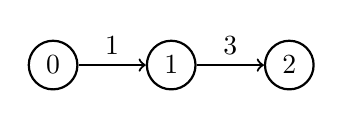
\begin{tikzpicture}[node distance={15mm}, thick, main/.style = {draw, circle}] 
                \node[main] (1) {0};
                \node[main] (2) [right of=1] {1};
                \node[main] (3) [right of=2] {2};
                \draw[->] (1) -- node[above] {1} (2);
                \draw[->] (2) -- node[above] {3} (3);
            \end{tikzpicture}
        \end{minipage}
        \begin{minipage}{\textwidth}
            \centering
            \vspace{0.2cm}
            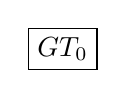
\begin{tikzpicture}[node distance={15mm}, main/.style = {draw, rectangle}] 
                \node[main] (0) {${GT_{0}}$};
            \end{tikzpicture}
        \end{minipage}
    \end{minipage}%
    \begin{minipage}[b]{.5\textwidth}
        \centering
        \begin{minipage}{\textwidth}
            \centering
            \begin{tikzpicture}[node distance={15mm}, thick, main/.style = {draw, circle}] 
                \node[main] (0) {0};
                \node[main] (1) [right of=1] {1};
                \node[main] (2) [right of=2] {2};
                \draw[->] (0) to [in=135, out=45] node[above] {1} (2);
                \draw[->] (0) -- node[above] {1} (1);
                \draw[->] (1) -- node[above] {3} (2);
            \end{tikzpicture}
        \end{minipage}
        \begin{minipage}{\textwidth}
            \centering
            \vspace{0.2cm}
            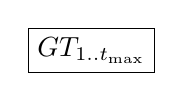
\begin{tikzpicture}[node distance={15mm}, main/.style = {draw, rectangle}] 
                \node[main] (0) {${GT_{1..{t_{\max}}}}$};
            \end{tikzpicture}
        \end{minipage}
    \end{minipage}
    \caption{Graphe temporel $GT$}\label{fig:exemple_dijkstra}
\end{figure}

Pour Dijkstra, au temps 0, le seul noeud visitable est le noeud 1 et va donc passer par le lien \link{0}{1}{1}, une fois au noeud 1, le seul lien accessible à parcourir est le lien \link{1}{3}{2}, et il va donc prendre ce chemin, pour un coût total de 4.
Alors que nous pouvons facilement voir que le plus court chemin est en fait d'attendre sur 0, puis de prendre le lien \link{0}{1}{2}, pour un coût total de 2.

Cependant, nous avons récemment pensé à une nouvelle structure de données.
Désormais, plusieurs liens peuvent exister entre 2 noeuds, mais ils ne sont pas tous actifs en même temps.
Nous allons donc avoir des liens fantômes qui remplacent les liens supprimés, équivalents à la distance réelle plus l'attente nécessaire.

Cela va permettre de ne pas avoir besoin de regarder dans le futur pour calculer les chemins, tout en calculant quand même la vraie distance minimale,
et ainsi rendre beaucoup plus de parcours de graphes adaptables temporellement, notamment Dijkstra, Bellman-Ford, A*, Johnson, etc\dots

\begin{algorithm}[H]
\caption{Construction de la structure de données}
%Pour chaque lien (A --p--> B) supprimé d'un temps t à t',
%Pour chaque pas de temps de tx de t à t', on ajoute un lien (A --p+(t'-tx)--> B, tx) qui sera disponible au temps tx, seulement.
\begin{algorithmic}
\State $NouveauGraphe \gets \emptyset$
\For{$lien \gets$ Attaque.liensBloqués()}
    \State $t_{BlocageInitial} \gets$ $lien$.tempsBlocageInitial()
    \State $t_{BlocageFinal} \gets$ $lien$.tempsBlocageFinal()
    \For{$t \gets$ $t_{BlocageInitial}$ to $t_{BlocageFinal}$}
        \State $LienFantome \gets$ new LienFantome($lien.origine$, $lien.destination$)
        \State $LienFantome.poids \gets$ $lien.poids + (t_{BlocageFinal} - t)$
        \State $NouveauGraphe$.ajouterLienDisponibleA($LienFantome$, $t$)
    \EndFor
\EndFor
\end{algorithmic}
\end{algorithm}

Cette solution est la plus compliquée à implémenter, mais aussi très prometteuse.
Notre implémentation prototype montre déjà des résultats encourageants, mais il faut encore vérifier la validité des résultats et tester la performance sur des graphes plus grands.

\subsection{Nouvelles attaques}\label{subsec:nouvelles_attaques}
L'équipe Complex Networks du Lip6 a travaillé sur des coupes de graphes, c'est-à-dire le diviser en sous-composantes connexes, et leur but est de minimiser le nombre de liens à supprimer pour obtenir cette division.
Nous allons récupérer certaines de leurs coupes calculées, et les utiliser pour attaquer le graphe, afin de voir si elles sont pertinentes.
\todo{reformuler}
\todo{lien vers complex networks}
\todo{préciser coupes de Paris très efficaces}

\subsection{Modification de la mesure}
L'efficacité est une mesure intéressante, mais elle ne prend pas en compte la variation comparée à un graphe non-attaqué.
Nous pourrions donc modifier la mesure pour prendre en compte cette variation, afin de comparer le changement d'efficacité plûtot que l'efficacité elle-même.